\chapter{Boost library}
\label{chap:Boost-library}
\label{sec:Boost-library}

There are three kinds of libraries:
\begin{enumerate}
  \item Header-only libraries: dependencies are resolved at compile time
  \item Static libraries: dependencies are resolved at link time
  \item Dynamic (shared) libraries: dependencies are resolved at run-time
\end{enumerate}

Boost is not a single library, but a collection of many libraries (58
libraries in Boost 1.32.0), written by different authors. Many of Boost
components are header-only libraries. 

The Boost organization has a standard for adding a new library into Boost. Boost
makes C++ programming more elegant, robust and productive.

Many libraries in Boost are now a part of the Standard Template Library (STL) in
the new C++ specification, C++11. So, it's suggested to use C++11 features if
possible. 

NOTE: Any thing from the STL, it starts with \verb!std::!; while those from
Boost, it starts with \verb!boost::!. 

Comparison of features in C++11 STL vs. Boost
\footnote{\url{http://stackoverflow.com/questions/8851670/relevant-boost-features-vs-c11}}
\begin{enumerate}
  \item Boost.Lambda = lambda expression (in non-polymorphic case) 
  
  NOTE: Boost.Lambda is still useful for polymorphic lambdas
  
  \item Chrono (Sect.\ref{sec:Boost.Chrono}) = now part of C++11 \verb!#include!
  \verb!<chrono>! - Sect.\ref{sec:chrono-header-file}
   
    
  \item Foreach (\verb!BOOST_FOREACH!) = range-based for
  
  \item Functional/Forward = perfect forwarding (rvalue references, variadic
  templates, std::forward)
  
  NOTE: Boost Functional/Hash
  \footnote{\url{http://www.boost.org/doc/libs/1_53_0/doc/html/hash.html}}
  contains some functions not found in C++11, e.g. \verb!hash_combine!
  
  NOTE: A large part of Boost MPL library
  \footnote{\url{http://www.boost.org/doc/libs/1_53_0/libs/mpl/doc/index.html}}
  can be replaced by using variadic templates
  
  \item Local function = Lambda expression

  \item Some common use cases of Boost Lexical-cast
  \footnote{\url{http://www.boost.org/doc/libs/1_53_0/doc/html/boost_lexical_cast.html}}
  can be replaced by \verb!std::to_string! and \verb!std::stoX!.
  
  \item Min-Max = std::minmax, \verb!std::minmax_element!
  \item Move = rvalue reference
  \item Ratio = \verb!std::ratio!
  \item static assert = \verb!static_assert!
  \item Thread = \verb!#include <thread>!
  \item Typeof = 'auto', 'decltype' keywords
  \item Value initialization = List-initialization
  \item Array = \verb!std::array!
  \item Bind = \verb!std::bind!
  \item Enable If = \verb!std::enable_if!
  \item Function = \verb!std::function!
  \item Member function = \verb!std::mem_fn!
  \item Random = \verb!#include <random>!
  \item Ref  = \verb!std::ref!, \verb!std::cref!
  \item Regex = regular expression \verb!#include <regex>!
  
  NOTE: C++11 doesn't support Perl5 regular expression like Boost Regex. Certain
  \verb!regex! interface members (e.g. \verb!boost::basic_regex<>::empty()!) is
  exactly matched with Boost Xpressive; and play much more nicely with Boost
  String Algorithms, which doesn't a C++11 standard counterparts yet.
  
  \item Utility, e.g. \verb!boost::result_of<>! =  \verb!std::result_of!
  
  \item Smart Pointer = \verb!std::unique_ptr!, \verb!std::shared_ptr!,
  \verb!std::weak_ptr! (KEEP \verb!boost::intrusive_ptr!)
  
  NOTE: \verb!std::unique_ptr! is part of TR1 (Sect.\ref{sec:unique_ptr}).
  
  \verb!const std::unique_ptr! replaces the use of \verb!boost::scoped_ptr! and
  \verb!boost::scoped_array!
  
  \item Swap (swapping arrays) = now part of C++11 \verb!std::swap!
  
  \item Tuple = now part of C++11 \verb!std::tuple! - Sect.\ref{sec:std::tuple}
  
  \item Type Traits = now part of C++11 \verb!#include <type_traits>! -
  Sect.\ref{sec:type_traits-header}
  
  NOTE: C++11 doesn't support \verb!call_traits! like Boost Type Traits.
  
  \item Unordered = \verb!#include <unordered_set>!, \verb!#include!
  \verb!<unordered_map>!
   
  \item Range = \verb!std::tie!, \verb!std::begin!
\end{enumerate}


\section{Overview}

\subsection{What is Boost.Build (b2)?}
\label{sec:Boost.Build}
\label{sec:b2-program}

Boost.Build is a high-level build system which makes it as easy as possible to
manage C++ projects.
The idea is to use configuration files just as much as necessary to build a
program.
Boost.Build supports many compilers out of the box and knows how to use them.
\url{https://boostorg.github.io/build/}

\url{https://www.boost.org/doc/libs/1_64_0/tools/build/tutorial.html}

Boost.Build translates options in configuration files to command line options
expected by the selected compiler.

However, regardless as nice as it sounds, Boost.Build can only be used for C++ and C projects.
Boost.Build doesn't know how to use other compilers like a Java compiler. 


ORIGINAL APPLICATATION:
Boost.Build was created to build and install the Boost C++ libraries easily with
different compilers on different platforms.

\url{https://www.boost.org/doc/libs/1_63_0/tools/build/tutorial.html}

Boost.Build uses a programm called {\bf b2} (previously it is called {\bf
bjam}). b2 looks for configuration files, reads them and builds a project
accordingly. b2 does indeed look for two more configuration files when it
starts.
\begin{enumerate}
  
  \item site-config.jam: used to set options for an entire system. This file is
  controlled by sys-admin, and not everyone can modify it.
  
In Boost, the file name is \verb!project-config.jam! file [which is generated by ./bootstrap.sh script]
\begin{verbatim}
./bootstrap --prefix=/path/to/install
\end{verbatim}

  \item \verb!user-config.jam!: b2 also looks for a file user-config.jam in a user's home director
  
As the file user-config.jam can be maintained by users it is probably used more
often than site-config.jam.
 
As these configuration files do not belong to a project but to a machine or a
user on a machine they are allowed to contain machine-specific options.

\end{enumerate}


\begin{mdframed}


The Boost.Build engine is derived from an earlier build tool called Perforce
Jam.
Originally, there were just minor changes, and the filename was bjam.
With more changes, as of Boost 1.47.0, the official name of the executable was
changed to b2. A copy named bjam is still created for compatibility, but you are
encouraged to use the new name in all cases.

\end{mdframed}


The configuration file b2 is looking for is a file with extension \verb!*.jam!,
called Jamfile.jam.


When the build system is loaded it also prepares itself to use a certain
compiler, linker and maybe other tools required to build a project. Boost.Build
refers to these programs as a {\bf toolset}. As of today there are more than 10 toolsets supported.

If no command line option is used to start b2 the build system tries to find a
toolset it can use automatically. To manually select a toolset, run ./b2 with option
toolset=something.

\begin{verbatim}
#If you want GCC to be used 
./b2 toolset=gcc


warning: No toolsets are configured.
warning: Configuring default toolset "msvc".
warning: If the default is wrong, your build may not work correctly.
warning: Use the "toolset=xxxxx" option to override our guess.
warning: For more configuration options, please consult
warning: http://boost.org/boost-build2/doc/html/bbv2/advanced/configuration.html
\end{verbatim}

\subsection{example *.jam file: simplest}

The programming language Boost.Build is based on knows only one data type:
Everything is a list of strings. A list can be empty or contain one or more
strings.


It means create an 'exe' file, name 'hello', using source file 'hello.cpp'
\begin{verbatim}
exe hello : hello.cpp ; 
\end{verbatim}
Boost.Build will detect the proper toolset, e.g. GCC in this case.

Boost.Build provides a lot of built-in rules and {\bf exe} is one of them, which
is a function. The function exe is called with two parameters each one a list
containing one string. In the Jamfile above the function exe is called with the
two parameters hello and hello.cpp.

It is possible to use quotes
\begin{verbatim}
exe "hello" : "hello.cpp" ; 
\end{verbatim}
There is no special character to separate a rule name and the first parameter, i.e. just a space is enough.
Then, a colon must be used to separate other parameters; and a space must be followed. 

IMPORTANT: Without spaces around tokens b2 won't be able to parse Jamfiles correctly.

Another important rule is lib. It is used to build a library.
\begin{verbatim}
lib world : world.cpp ; 
\end{verbatim}
By default, a shared library is built.
\begin{verbatim}
lib world : world.cpp : <link>static ; 
\end{verbatim}


\subsection{example *.jam file: <variant> option}

The fourth parameter contains features which are used by default but which can be overwritten.
\begin{verbatim}
exe hello : hello.cpp : <variant>release ; 

exe hello : hello.cpp : : <variant>debug <variant>release ; 
\end{verbatim}
As a program can't be a debug and a release version at the same time <variant> must be set in the default values, 
the <variant> feature needs to be set twice to debug and release.

Only then Boost.Build understands that two versions of hello.exe should be built.

\subsection{: <define> option}
\begin{verbatim}
exe hello : hello.cpp : <define>WIN32 <define>_WIN32 : <variant>debug <variant>release ; 

\end{verbatim}

The feature <define> is used to define preprocessor directives

A debug version optimized for speed, a debug version with no optimization, a release version optimized for speed and a release version with no optimization.
All of these versions are built in seperate directories which are automatically created.
\begin{verbatim}

exe hello : hello.cpp : : <variant>debug <variant>release <optimization>speed <optimization>off ; 

\end{verbatim}


A variant is a debug or release version of a program. For each variant another
directory is used to build a program - again for the reason not to overwrite
files produced by another variant.

By default the debug variant is used. If you want a release version to be
created you can specify the variant on the command line with b2 variant=release
or, even simpler, b2 release .

There are not only toolset-specific directories but also variant-specific
directories.


If you don't want to specify the variant on the command line but want to build
release versions of hello.exe by default the Jamfile has to be changed.
\begin{verbatim}
exe hello : hello.cpp : <variant>release ; 
\end{verbatim}

\subsection{How to install}

There is a script \verb!./bootstrap.sh! which accepts a number of command-line options to help creating 
\begin{verbatim}
JAM_CONFIG_OUT=project-config.jam
\end{verbatim}
file. 

\begin{verbatim}
./bootstrap.sh --prefix=/usr/local/boost-1.68.0

./bootstrap.sh --prefix=/packages/boost/1.68.0 --with-python-version=3.6

\end{verbatim}

or check python location, e.g. /packages/anaconda3/3.4.1/bin
\begin{verbatim}
./bootstrap.sh  --prefix=/packages/boost/1.68.0 \
     --with-python=/packages/anaconda3/3.4.1/bin/python3
     --with-python-version=3.6
     --with-python-root=/packages/anaconda3/3.4.1/

\end{verbatim}
or just run with 
\begin{verbatim}
./bootstrap.sh  --prefix=/packages/boost/1.68.0 --with-python-version=X.Y
\end{verbatim}


Then, we can modify this file accordingly. In earlier version of Boost, they
mentions the file \verb!user-config.jam!.
NOTE: We can either rename to the oldname by editing \verb!bootstrap.sh!
\begin{verbatim}
//change this
cat > project-config.jam <<EOF

//to
cat > user-config.jam <<EOF
\end{verbatim} 
or to use your own file we pass
\begin{verbatim}
./bjam --user-config=user-config.jam
\end{verbatim}

NOTE: We should use \verb!project-config.jam!, rather than
\verb!user-config.jam!.


Finally, to build, we run
\begin{verbatim}
sudo ./b2 -d+2  install
\end{verbatim}

 \url{https://lists.boost.org/Archives/boost/2017/10/239485.php}
\begin{verbatim}
On a not entirely unrelated note, Rene Rivera has added a new feature 
<cxxstd> to Boost.Build that controls the C++ standard in use. So for 
instance, instead of the old 
    b2 libs/mylib/test toolset=gcc cxxflags=-std=c++11 
one can now use 
    b2 libs/mylib/test toolset=gcc cxxstd=11 
In addition to being more convenient, this also allows several invocations 
to be combined into one: 
    b2 libs/mylib/test toolset=clang cxxstd=03,11,14,1z 
\end{verbatim}
\url{https://gist.github.com/dennycd/5890475}

\subsection{-- explains}

As \verb!b2! (Boost.Build) is used, it loads the first jam file
\verb!boost-build.jam!, regardless from which Boost library subfolder. It allows us to choose 
which Boost.Build installation to use, unless overriden via command-line options, and
\begin{verbatim}
BOOST_BUILD ?= tools/build/src
\end{verbatim}
The file 
\begin{verbatim}
$BOOST_BUILD/build-system.jam
\end{verbatim}
tells the default toolset, based on the O/S.

In Mac O/S, Clang is the default; while in Linux, GCC is the default. 


IMPORTANT: a C++ library compiled with GCC is not compatible with Clang and
vice-versa. So, you won’t be able to use a Clang build Boost with GCC.
 
\subsection{-- project-config.jam file}

If you use the default setting, the build is straightforward, run boostrap.sh to generate 
project-config.jam file 
\begin{verbatim}

# default (install all Boost libraries)
./bootstrap.sh --prefix=/usr/local/boost-1.68.0

# (select some libraries)
./bootstrap.sh --prefix=/usr/local/boost/1_68_0 --with-libraries=chrono,system,thread,timer,signals,random,date_time,coroutine

#  it's probably better to use the dedicated cxxstd feature. 
# You could add it to project-config.jam as <cxxstd>14, or pass it when building, as in b2 cxxstd=14.

# compile with C++14 standard --> some functions in Boost libraries are only available with C++14
sudo ./b2 cxxstd=14 install

\end{verbatim}

If you want to use a different GCC version, first be sure that you have GCC 8
installed and available in your path.

\begin{verbatim}

#edit project-config.jam [see below]

sudo ./b2 cxxflags=-std=c++17 install
\end{verbatim}

Edit file: Feel free to change 8.1 to match the version of GCC you have 

\begin{verbatim}
#if ! darwin in [ feature.values <toolset> ]
#{
#    using darwin ;
#}

#project : default-build <toolset>darwin ;
 
#using gcc : 8.1 : /usr/local/gcc-8.1/bin/g++-8.1 : <cxxstd>14 ; # C++ 14

using gcc : 7.3 : /packages/gcc/7.3/bin/gcc : <cxxflags>-std=c++14 <link>=shared ; # C++ 14

#using gcc : 8.1 : /usr/local/gcc-8.1/bin/g++-8.1 : <cxxflags>-std=c++14 ; # C++ 14

import python ;
#if ! [ python.configured ]
#{
#    using python : 3.6 : /packages/anaconda3/5.2.0 ;
#}
using python
    : 3.6                   # Version
    : /packages/anaconda3/5.2.0/bin/python # Python path
    : /packages/anaconda3/5.2.0/include/python3.6m/  # include path
    : /packages/anaconda3/5.2.0/lib  # lib paths
;

\end{verbatim}
\url{https://github.com/boostorg/system/issues/26}

\url{https://boostorg.github.io/build/manual/develop/index.html}

NOTE: We can define as many variants/toolset as we like, with the tilde to delineate a variation
\begin{verbatim}
using gcc : 5 : g++-5 : ; # default is C++ 98
using gcc : 5~c++03 : g++-5 : <cxxflags>-std=c++03 ; # C++ 03
using gcc : 5~gnu03 : g++-5 : <cxxflags>-std=gnu++03 ; # C++ 03 with GNU
using gcc : 5~c++11 : g++-5 : <cxxflags>-std=c++11 ; # C++ 11
using gcc : 5~c++14 : g++-5 : <cxxflags>-std=c++14 ; # C++ 14
\end{verbatim}

and when we run with \verb!./b2! we can select 
\begin{verbatim}
# toolset name first (gcc) and then dash (-) before the version+variation (5~c++14)
b2 toolset=gcc-5 stage
b2 toolset=gcc-5~c++14 stage
\end{verbatim}

ISSUE with Anaconda Python in project-config.jam
\begin{verbatim}
using python : 3.6 : /home/myUser/anaconda3 ; 

\end{verbatim}
If we build
\begin{verbatim}
sudo ./b2 --with-python -j8 install
\end{verbatim}
then an error
\begin{verbatim}
./boost/python/detail/wrap_python.hpp:50:11: fatal error: 
pyconfig.h: No such file or directory
# include <pyconfig.h>
          ^~~~~~~~~~~~
compilation terminated.
\end{verbatim}
SOLUTION: we need to use
\begin{verbatim}
C_INCLUDE_PATH /packages/anaconda3/5.2.0/include/python3.6m/
CPLUS_INCLUDE_PATH /packages/anaconda3/5.2.0/include/python3.6m/
\end{verbatim}
\url{https://stackoverflow.com/questions/54152667/how-to-fix-pyconfig-h-not-found-with-anaconda}

EDIT THE FILE: Btw, to enable MPI support, we add to the file project-config.jam
\begin{verbatim}
using mpi ; #to enable MPI support

#or tell it where to look for the file as well
# check <boost>/build/v2/tools/mpi.jam

using mpi : /usr/local/mpich2-1.0.4/bin/mpiCC;
\end{verbatim}
\url{https://www.boost.org/doc/libs/1_61_0/doc/html/mpi/getting_started.html}


EDIT THE FILE: TO compile with python 3
\begin{verbatim}
   using python : 3.5 :  /path/to/python/root : /path/to/python/include : /path/to/python/libs ;
\end{verbatim}
[NOTE: In Windows, use \verb!\\! for path]

Example:
\begin{verbatim}
  // early name when it is a folk of JAM build system
./bjam install --prefix=PREFIX

 // now is b2 as it is very much different from the original 'JAM'
./b2 install --prefix=PREFIX


./b2 toolset=clang cxxflags="-stdlib=libc++ -std=c++11" linkflags="-stdlib=libc++ -std=c++11" 

./b2 toolset=gcc cxxflags=-std=c++14 --prefix=/packages/boost/1.6.80s --with-mpi
\end{verbatim}

Here we use PREFIX=\verb!/usr/local/boost!. Other useful options
\begin{verbatim} 
  //to provide more details
--debug-configuration 
  //to force enable MPI
--with-mpi
  //suppress the warning message when no MPI is supported
--without-mpi

  // to build only Boost.Python
--with-python
\end{verbatim}


HOW TO USE: here we link to two different libraries inside boost (e.g. boost:system and boost::filesystem)
\begin{verbatim}
g++-8.1 -std=c++17 -I /usr/local/boost-1.68.0/include -L /usr/local/boost-1.68.0/lib test.cpp -o test -lboost_system -lboost_filesystem

clang++ -std=c++17 -I /usr/local/boost-1.68.0/include -L /usr/local/boost-1.68.0/lib test.cpp -o test -lboost_system -lboost_filesystem

\end{verbatim}

\url{https://solarianprogrammer.com/2018/08/07/compiling-boost-gcc-clang-macos/}

You may want to install first
\begin{enumerate}
  \item bzip2 header files: 
  \begin{verbatim}
  #RED-HAT
  sudo yum install bzip2-devel.x86_64
  
  #UBUNTU
  \end{verbatim}
  NOTE: To search for package names, if you don't remember exactly the name in
  RedHat
  \begin{verbatim}
  sudo yum search bzip
  \end{verbatim}
  
  \item python header files:
  \begin{verbatim}
  sudo yum install python-devel.x86_64
  \end{verbatim}
  
  \item You may also want to modify the \verb!user-config.jam! file
  
  Copy the template from
  \begin{verbatim}
  boost_<version>/tools/build/v2/user-config.jam

OR
  boost/tools/build/user-config.jam

  \end{verbatim}
  into boost source directory
  
\end{enumerate}

The default installation folder is /usr/local/
\begin{verbatim}
Boost_DIR=/usr/local/boost_1_53_0
Boost_INCLUDE_DIR=/usr/local/boost_1_53_0/include/

Boost_LIB_DIR=/usr/local/boost_1_53_0/lib
\end{verbatim}
For many of the libraries in Boost, we only need the header files. However, some
requires the compiled shared libraries as well.

\subsection{Link your code agains boost}


If your code use Boost MPI, then you need to link against \verb!boost_mpi! and
\verb!boost_serialization!
\begin{verbatim}
mpic++ your_code.cpp   \
   -Llibdir -lboost_mpi-gcc-mt-1_35 -lboost_resialization-gcc-d-1_35.a
\end{verbatim}
If you also want to use Python-bindings for Boost.MPI, then
\begin{verbatim}
... 
-lboost_mpi_python-gcc-mt-1_35
\end{verbatim}
to your link command. This is necessary only if you register C++ types and use
skeleton/content mechanism (i.e. how to transfer large data structures
created in C++ to be used in Python code) from Python.

\section{a new way of using Boost with CMake}


Now for every Boost library there is a *.cmake file) instead of the one from CMake distribution


\section{boost::spirit (format data, parse data)}
\label{sec:boost_spirit}


Spirit was added to Boost since Boost 1.30.0 (March, 19th, 2003). The code base
of Spirit 1.8.x becomes \verb!Spirit.Classic! component in Spirit 2.x. 
\begin{itemize}
  \item Spirit 2.0 was added to Boost 1.37.0
  \item Spirit 2.1 was added to Boost 1.41.0:
  \item \ldots 
  \item Spirit 2.5 was added to Boost 1.47.0
  \item Spirit 2.5.1 was added to Boost 1.48.0
\end{itemize}

Spirit 2.5.1 has 4
components:\footnote{\url{http://boost-spirit.com/home/wp-content/uploads/2010/05/spirit_presentation.pdf}}
\begin{enumerate}
  \item boost::spirit::qi    (parsing input)
  \item boost::spirit::karma (generating output)
  \item boost::spirit::lex   (a lexer)
  \item boost::spirit::classic (old-parsing input). Any
existing code either uses the old Spirit (example:
Sect.\ref{sec:boost_spirit_classic}), or need to update the header files in
\begin{verbatim}
$BOOST_ROOT/boost/spirit/include
\end{verbatim} 
with \verb!classic_! prefix in the
names. E.g. 
\begin{verbatim}
#include <boost/spirit/include/core.hpp>
\end{verbatim}
becomes 
\begin{verbatim}
#include <boost/spirit/include/classic_core.hpp>
\end{verbatim}
and use the new namespace \verb!boost::spirit::classic!.

\end{enumerate}

\subsection{Lexer vs. Parser}

{\bf A lexer vs. A parser}: a lexer converts a sequence of characters into a
sequence of {\it tokens}. A lexer often exist as a single function which is
called by the parser. A token is a string of one or more characters that can be
classified into {\it token-type}. E.g.: 'sum'=identifier, '=' is assigment
operator, '3' or '2'=integer literal, ';' = end of statement. To define a token,
we can use {\it regular expressions}.

To interpret the data (in any form), and convert it into another form
using, the tool is called a {\it parser}. The parser can check if the input has
a correct format (in the case of file I/O), or a correct syntax (in the case of a
scripting language or programming language).


\subsection{Grammar presentation}

By defining a proper grammar specification, it can tell whether input follow the
grammar or not. What we want to parse can be anything (from email, command
lines, scritting languages, etc.). Languages are often ambiguous by nature. To
avoid this ambiguity (as much as we can), programming language are often
designed as {\bf context-free grammar} (CFG).

The rules are called Extended Backus-Nauer Form (EBNF) production rules. The
grammar describes both input and output. There are different ways to define a
grammar specification. The two major families of approaches are bottom-up
parsing and top-down parsing. It's expected that the language to be parsed is
{\bf context-free grammar}, i.e. the production rule is in the form
$V\rightarrow w$ ($w$ can be empty or a string of terminals or non-terminals,
$V$ is single non-terminal symbol).
\begin{enumerate}
  \item Top-down parsing: LL parser (or LL(k) parser if it use $k$ tokens of
  lookahead when parsing the input: parse from Left to Right, and construct
  Leftmost derivation
  tree)\footnote{\url{http://en.wikipedia.org/wiki/LL_parser}}. 
  
  Recursive descent parser is a kind of top-down parser that works only for
  LL($k$) grammars, built from a set of mutually recursive procedures (or
  non-recursive equivalent), each procedure implement one of the production rule
  of the grammar. It's pretty to implement using functional languages (Haskell,
  Lisp, etc.). \textcolor{red}{C and C++ parser of GCC uses this approach}.
  
  Tools to generate LL parsers are ANTLR (which can generate parser in C,
  C\#, Java, JavaScript, Objective-C, Perl, Ada95,
  etc.\footnote{\url{http://en.wikipedia.org/wiki/ANTLR}}),
  \verb!boost::spirit!.

  \item Bottom-up parsing: LR parser
  (Donald Knuth invented LR parser (Left-to-Right, Rightmost derivation) in
  1965). Variants of LR parser are LALR parser (Look-Ahead LR parser: done by
  shift-reduce parser), SLR parser (Simple LR parser), both proposed by Frank
  DeRemer in 1969 to avoid using large memory.
  
  Tools to generate LALR parsers are YACC, Bison
\end{enumerate}
NOTE: Understanding righe-derivation is harder than left-derivation. 

\verb!boost::spirit! is a recursive descent parser; with
\verb!boost::spirit::qi! is a fully object-oriented LL(k) parser and
lexical analyzer. Spirit treats both processes virtually identical. In
\verb!boost::spirit::qi!, a {\bf parser} is a small object that know how to
parse a particular string.  Traditionally, \verb!lex/flex!/ \verb!yacc/bison!
are widely used tools. The grammar can be built using primitive parsers, and
can be combined using overloadeed C++ operators. 

A grammar always start with the first parser, whose associated attribute is the
{\bf abstract syntax tree} (AST), which is a tree representation of the
syntactic structure of the source code.

An example of LL(1) from, terminals are expressed in quotes
{\small \begin{verbatim}
 program = block "." .
 
 block =
     ["const" ident "=" number {"," ident "=" number} ";"]
     ["var" ident {"," ident} ";"]
     {"procedure" ident ";" block ";"} statement .
 
 statement =
     ident ":=" expression
     | "call" ident
     | "begin" statement ";" {statement ";"} "end"
     | "if" condition "then" statement
     | "while" condition "do" statement .
 
 condition =
     "odd" expression
     | expression ("="|"#"|"<"|"<="|">"|">=") expression .
 
 expression = ["+"|"-"] term {("+"|"-") term} .
 
 term = factor {("*"|"/") factor} .
 
 factor =
     ident
     | number
     | "(" expression ")" .
\end{verbatim}}

A C implementation of a parser for the above grammar using recursive descent
parser approach
\lstset{language=C,
numberstyle=\footnotesize,
basicstyle=\ttfamily\footnotesize,
frame=shadowbox,
breaklines=true
}
\begin{lstlisting}
typedef enum {ident, number, lparen, rparen, times, slash, plus,
    minus, eql, neq, lss, leq, gtr, geq, callsym, beginsym, semicolon,
    endsym, ifsym, whilesym, becomes, thensym, dosym, constsym, comma,
    varsym, procsym, period, oddsym} Symbol;
 
Symbol sym;
void getsym(void);
void error(const char msg[]);
void expression(void);
 
int accept(Symbol s) {
    if (sym == s) {
        getsym();
        return 1;
    }
    return 0;
}
 
int expect(Symbol s) {
    if (accept(s))
        return 1;
    error("expect: unexpected symbol");
    return 0;
}
 
void factor(void) {
    if (accept(ident)) {
        ;
    } else if (accept(number)) {
        ;
    } else if (accept(lparen)) {
        expression();
        expect(rparen);
    } else {
        error("factor: syntax error");
        getsym();
    }
}
 
void term(void) {
    factor();
    while (sym == times || sym == slash) {
        getsym();
        factor();
    }
}
 
void expression(void) {
    if (sym == plus || sym == minus)
        getsym();
    term();
    while (sym == plus || sym == minus) {
        getsym();
        term();
    }
}
 
void condition(void) {
    if (accept(oddsym)) {
        expression();
    } else {
        expression();
        if (sym == eql || sym == neq || sym == lss || sym == leq || sym == gtr || sym == geq) {
            getsym();
            expression();
        } else {
            error("condition: invalid operator");
            getsym();
        }
    }
}
 
void statement(void) {
    if (accept(ident)) {
        expect(becomes);
        expression();
    } else if (accept(callsym)) {
        expect(ident);
    } else if (accept(beginsym)) {
        do {
            statement();
        } while (accept(semicolon));
        expect(endsym);
    } else if (accept(ifsym)) {
        condition();
        expect(thensym);
        statement();
    } else if (accept(whilesym)) {
        condition();
        expect(dosym);
        statement();
    } else {
        error("statement: syntax error");
        getsym();
    }
}
 
void block(void) {
    if (accept(constsym)) {
        do {
            expect(ident);
            expect(eql);
            expect(number);
        } while (accept(comma));
        expect(semicolon);
    }
    if (accept(varsym)) {
        do {
            expect(ident);
        } while (accept(comma));
        expect(semicolon);
    }
    while (accept(procsym)) {
        expect(ident);
        expect(semicolon);
        block();
        expect(semicolon);
    }
    statement();
}
 
void program(void) {
    getsym();
    block();
    expect(period);
}
\end{lstlisting}  

\subsection{Change Logs}

\begin{enumerate}
  \item  Spirit::Qi V2.1 code changes: (1)
  \verb!qi::phrase_parse!, \verb!qi::phrase_format! do post-skip by default, (2)
  attributes is always the last parameter in the functions
  \begin{verbatim}
  qi::phrase_parse()
  qi::phrase_match() 
  karma::generate_delimited()
  match_delimited()
  \end{verbatim}
  
  \item Spirit::Qi V2.1.
  \url{http://www.boost.org/doc/libs/1_42_0/libs/spirit/doc/html/spirit/what_s_new.html}
  
  \item \ldots
  
  \item Spirit X3: the redesign of Spirit for C++11. Here, the
  simplicity of Spirit.Classic will be regained the porpularity (Spirit V2.x is
  more complex )
  \url{http://boost-spirit.com/home/2013/02/23/spirit-x3/}
\end{enumerate}

\subsection{Test a parser}

The library provides some free functions to make parsing easy
\begin{enumerate}
  \item boost::spirit::qi::parse(\ldots)
  \item \verb!boost::spirit::qi::phrase_parse!(\ldots): we need to use this if
  the grammar has a \verb!skip!-parser.
\end{enumerate}
which returns 'true' if parsing is successful.

\url{http://www.boost.org/doc/libs/1_41_0/libs/spirit/doc/html/spirit/advanced/indepth/parsers_indepth.html}
{\bf Parser} class is the base class for all parsers. This class doesn't really
know how to parse anything, but rely on the template parameter \verb!Derived! to
do the actual parsing which is a real parser. It uses the technique called
{Curiously Recurring Template Pattern} in template meta-programming circles.
\begin{lstlisting}
template <typename Derived>
struct parser
{
    struct parser_id;
    typedef Derived derived_type;
    typedef qi::domain domain;

    // Requirement: p.parse(f, l, context, skip, attr) -> bool
    //
    //  p:          a parser
    //  f, l:       first/last iterator pair
    //  context:    enclosing rule context (can be unused_type)
    //  skip:       skipper (can be unused_type)
    //  attr:       attribute (can be unused_type)

    // Requirement: p.what(context) -> info
    //
    //  p:          a parser
    //  context:    enclosing rule context (can be unused_type)

    // Requirement: P::template attribute<Ctx, Iter>::type
    //
    //  P:          a parser type
    //  Ctx:        A context type (can be unused_type)
    //  Iter:       An iterator type (can be unused_type)
    
    Derived const& derived() const {
        return *static_cast<Derived const*>(this);
    }
};
\end{lstlisting}

Using inheritance, we can avoid the overhead of virtual functions
(Sect.\ref{sec:overhead-of-virtual-function}), i.e. the required functions like
\verb!parse()! doesn't have to be in \verb!Parser! class, but its inheritance
will define it. The predefined {\it Derived} class in Boost.Spirit are
PrimitiveParser (Sect.\ref{sec:primitive_parsers}), UnaryParser
(Sect.\ref{sec:unary_parsers}), BinaryParser and NaryParser; and they need to
support
\begin{lstlisting}
bool parse(f, l, context, skip, attr)
\end{lstlisting}
The parser implementation is derived from \verb!boost::spirit::qi::primitive_parser<>!.

\begin{mdframed}
A \verb!Parser! is the most fundamental concept in Boost::Spirit::Qi, with a
member function \verb!parse()!, that accepts a first-last {\it ForwardIterator}
\footnotemark[1] {\bf pair} of the input (string need to be checked with
grammar) using the rule context \verb!context! and returns \verb!bool! as its
result (TRUE=parsing success, FALSE=failed).
\begin{verbatim}
p.parse(f, l, [context, [skip, [attr]]])
\end{verbatim}
with $f,l$ is the ForwardIterator pair (or two arguments as first/last iterator
pair), the parser's \verb!context! (e.g.
\verb!char_! or some complicated \verb!grammar!), \verb!skip! parser, and
\verb!attrib! is a compatible attribute where the parser is supposed to store
its result. [] means optional \footnotemark[2].

Upon entry the \verb!parse()! function, PrimitiveParser is required to do a
pre-\verb!skip! using the \verb!skipp! parser. It means that leading \verb!skip!
characters/tokens will be skipped prior to parsing, which is typically carried
out through a call to \verb!qi::skip_over(f,l,skip)!. However, only
PrimitiveParser is required to perform this step \footnotemark[3].

If parsing successfully, $f$ is incremented $N$ number of times, with $N$ is the
number of characters parsed ($N$ can be zero). If successfull, the parsed result
is assigned to \verb!attr!. If parsing failed, $f$ is reset to the position
before entering the parser function, and \verb!attr! is untouched.
\end{mdframed}
\footnotetext[1]{\url{http://www.sgi.com/tech/stl/ForwardIterator.html}}
\footnotetext[2]{\url{http://www.boost.org/doc/libs/1_41_0/libs/spirit/doc/html/spirit/qi/reference/parser_concepts/parser.html}}
\footnotetext[3]{\url{http://www.boost.org/doc/libs/1_41_0/libs/spirit/doc/html/spirit/qi/reference/parser_concepts/primitiveparser.html}}



To test parser without attribute
\begin{lstlisting}
#include <boost/spirit/include/support_utree.hpp>
#include <boost/spirit/include/qi.hpp>
#include <boost/spirit/include/phoenix_core.hpp>
#include <boost/spirit/include/phoenix_operator.hpp>
#include <boost/fusion/include/adapt_struct.hpp>
#include <boost/assert.hpp>
#include <iostream>
#include <string>
#include <cstdlib>

template <typename P>
void test_parser(
    char const* input, P const& p, bool full_match = true)
{
    using boost::spirit::qi::parse;

    char const* f(input);
    char const* l(f + strlen(f));
    if (parse(f, l, p) && (!full_match || (f == l)))
        std::cout << "ok" << std::endl;
    else
        std::cout << "fail" << std::endl;
}

template <typename P>
void test_phrase_parser(
    char const* input, P const& p, bool full_match = true)
{
    using boost::spirit::qi::phrase_parse;
    using boost::spirit::qi::ascii::space;
    
    char const* f(input);
    char const* l(f + strlen(f));
    if (phrase_parse(f, l, p, space) && (!full_match || (f == l)))
        std::cout << "ok" << std::endl;
    else
        std::cout << "fail" << std::endl;
}
\end{lstlisting}

If we want to test user-defined parser with user supplied attributes.
\begin{lstlisting}
template <typename P, typename T>
void test_parser_attr(
    char const* input, P const& p, T& attr, bool full_match = true)
{
    using boost::spirit::qi::parse;

    char const* f(input);
    char const* l(f + strlen(f));
    if (parse(f, l, p, attr) && (!full_match || (f == l)))
        std::cout << "ok" << std::endl;
    else
        std::cout << "fail" << std::endl;
}

template <typename P, typename T>
void test_phrase_parser_attr(
    char const* input, P const& p, T& attr, bool full_match = true)
{
    using boost::spirit::qi::phrase_parse;
    using boost::spirit::qi::ascii::space;

    char const* f(input);
    char const* l(f + strlen(f));
    if (phrase_parse(f, l, p, space, attr) && (!full_match || (f == l)))
        std::cout << "ok" << std::endl;
    else
        std::cout << "fail" << std::endl;
}
\end{lstlisting}

\subsection{Primitive parsers (boost::spirit::qi)}
\label{sec:primitive_parsers}

To help building complicated parsers, there are existing simple parsers written
in boost::spirit, Fig.\ref{fig:Boost_Spirit_parsers}, which makes heavy use of
template meta-programming and functors. Example
\begin{lstlisting}
#include <boost/spirit/include/qi_int.hpp>
using boost::spirit::qi::int_; // to recognize a string 
               // preresenting an integer

bool info = test_parser("+12345", int_); //integer parser

#include <boost/spirit/include/qi_real.hpp>
using boost::spirit::qi::double_;
using boost::spirit::qi::real_parser;

test_parser("+12345e6", double_); //double parser

real_parser<double, ts_real_policies<double> > ts_real;
test_parser("123,456,789.01", ts_real);
...
\end{lstlisting}
NOTE: Remember to link the code \verb!-I/path/to/boost/include-folder!.

Like other primitive parsers, \verb!int_, double_!, \ldots are just placeholder
symbols denoting the type of the parser component required to match the input. It means that they will be
compiled into real parser instances responsible for the actual matching of the
input. \verb!boost::spirit::compile! is the built-in facility to perform the
conversion of the parser expression into corresponding parser instance
\footnote{\url{http://www.boost.org/doc/libs/1_47_0/libs/spirit/doc/html/spirit/qi/quick_reference/qi_parsers.html}}.

\begin{enumerate}
  \item Character parsers:
  \url{http://www.boost.org/doc/libs/1_47_0/libs/spirit/doc/html/spirit/qi/quick_reference/qi_parsers/char.html}
  
  \item String parsers:
  \url{http://www.boost.org/doc/libs/1_47_0/libs/spirit/doc/html/spirit/qi/quick_reference/qi_parsers/string.html}
  
  \item \ldots
\end{enumerate}


\begin{figure}[hbt]
  \centerline{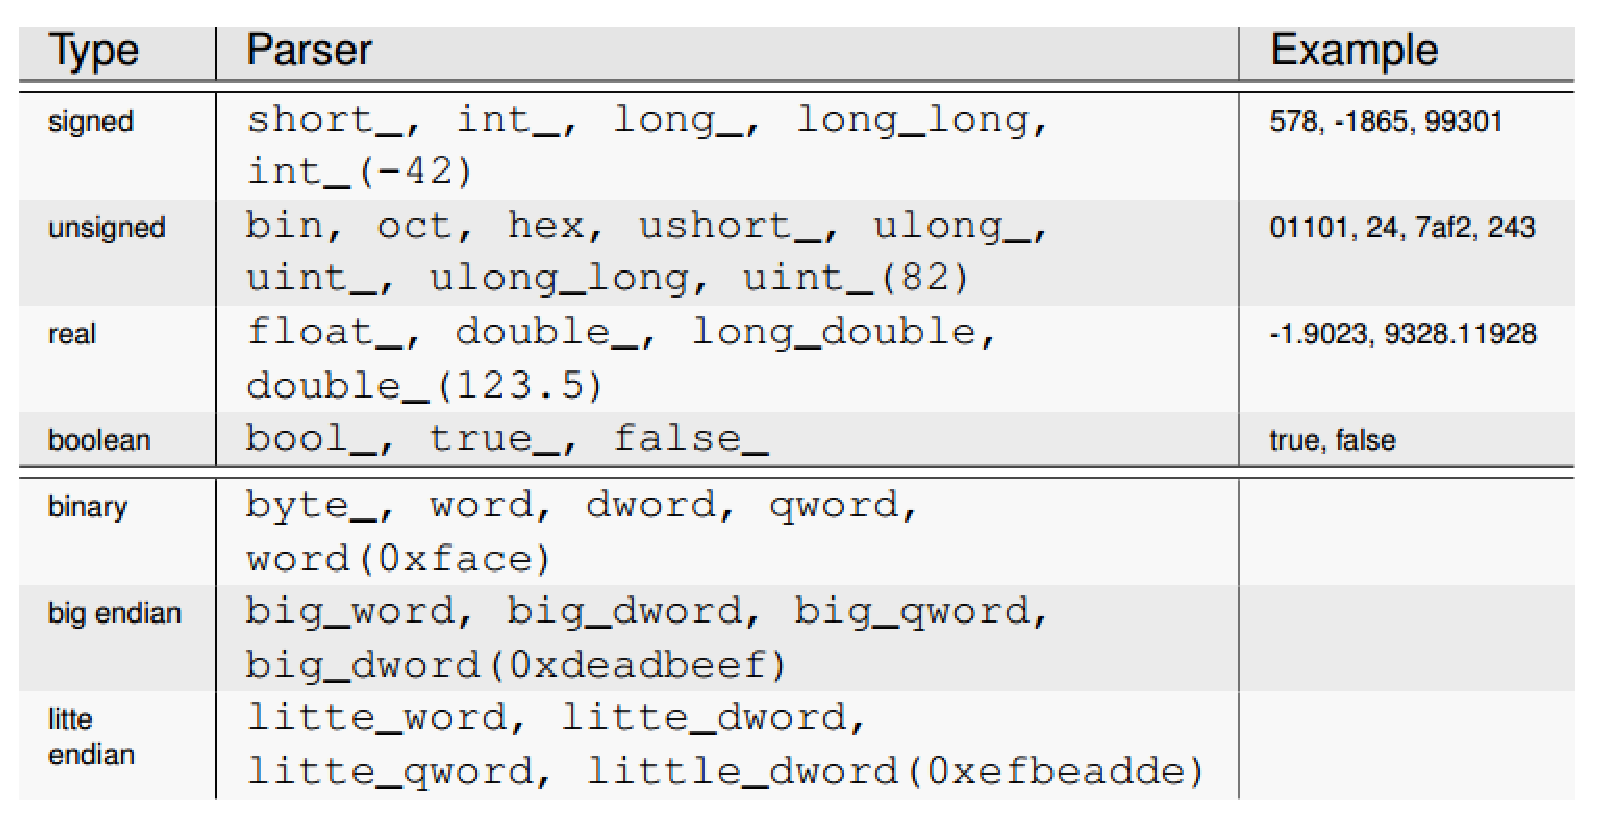
\includegraphics[height=5cm,
    angle=0]{./images/Boost_Spirit_parsers.eps}}
  \centerline{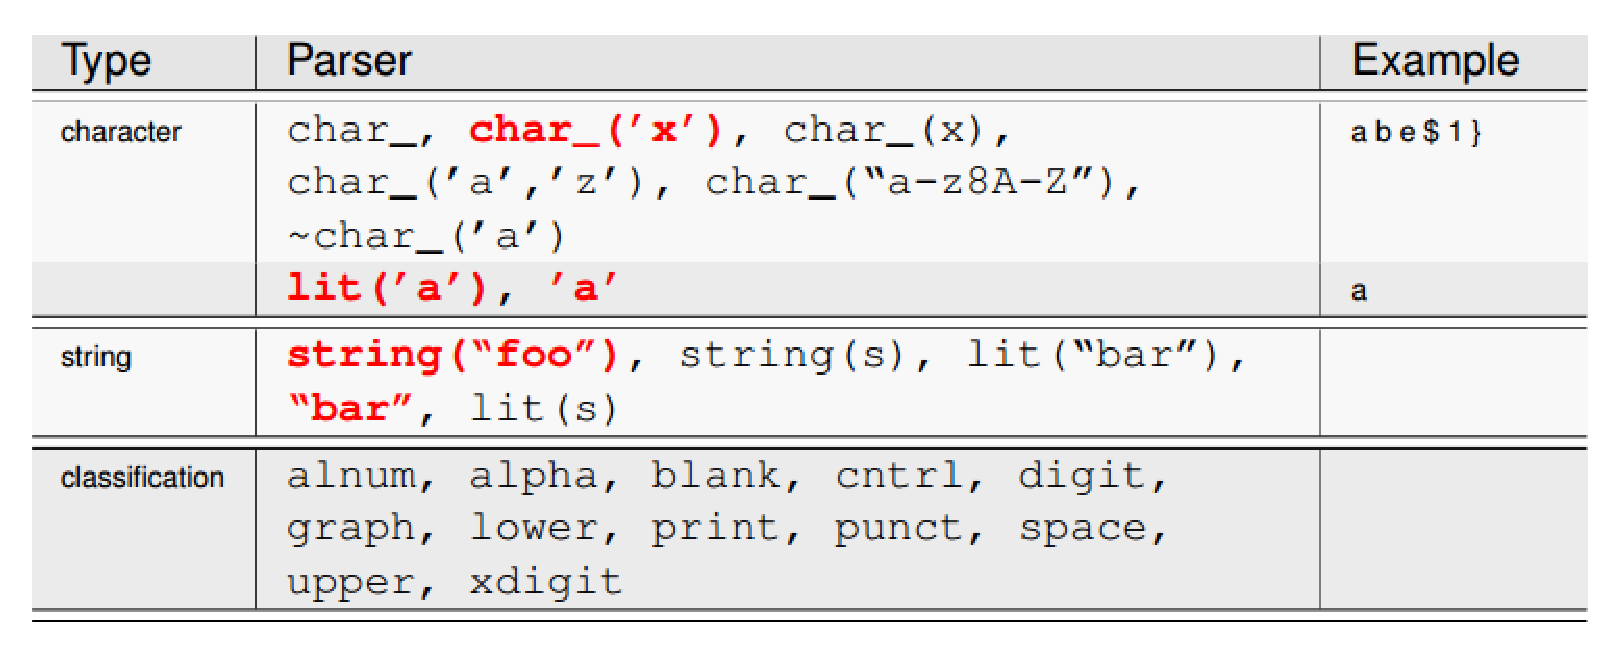
\includegraphics[height=4cm,
    angle=0]{./images/Boost_Spirit_parsers_2.eps}}
  \caption{Available parsers in Spirit::Qi}
  \label{fig:Boost_Spirit_parsers}
\end{figure}

\textcolor{red}{\bf Parsing characters and string need to be careful, due to
different ways to be done, and different character encoding namespace}.  The
possible choices are
\begin{verbatim}
boost::spirit::ascii
boost::spirit::iso8859_1
boost::spirit::standard
boost::spirit::standard_wide
\end{verbatim}
which are also brought into \verb!qi! sub-namespace
\begin{verbatim}
boost::spirit::qi::ascii
boost::spirit::qi::iso8859_1
boost::spirit::qi::standard
boost::spirit::qi::standard_wide
\end{verbatim}
Most of the time, we'll work with \verb!boost::spirit::qi::ascii!.

\textcolor{red}{\bf Character matching}: There are also important notices.
\verb!char_! is a boost::spirit::terminal (grammar[1]) that recognizes a single
character (an alphabet, a numeric, a comma, a dot, etc.), and return the
character as the associated attribute of type \verb!char!. To recognize a single
character, say 'a', we can use \verb!char_("a")!; or a single character (any
one from 'a' to 'z'), we can use \verb!char_("a-z")!. To recognize a single
character, but don't return it to the associated attribute, we use \verb!lit()!
parser.

\begin{verbatim}
//to match a single character, in variable 'ch'
char ch; ch='a';
bool info;

//we have 3 options (but associated attribute can be different)
info = qi::parse("a", ch);
info = qi::parse("a", lit(ch));
info = qi::parse("a", char_(ch));

//to match a single character literal, say 'c'
info = qi::parse('c', char_('c'));

// match any character, e.g. '+', '-' are also character
info = qi::parse('a', char_);
info = qi::parse('b', char_);

// alphabetic only (a-zA-Z)
info = qi::parse('a', alpha) ;

// alphanumeric (a-zA-Z0-9)
info = qi::parse('4', alnum);

//match a string
boost::spirit::qi::lit("some string") ; //string literal parser
\end{verbatim}
with \verb!info! is true for parsing successfully.


NOTE: These primitive parsers can be combined to build more complex parsers
(to be discussed at Sect.\ref{sec:boost_spirit::qi_user_defined_parser}). A good reference
is\footnote{\url{http://boost-spirit.com/home/articles/qi-example/creating-your-own-parser-component-for-spirit-qi/}}

\textcolor{red}{\bf Running the parser is simple}. What we need: (1) an input
string we want to parse, (2) the parser containing the grammar (primitie
parser, a combination of these primitive parsers using operators, or write your
own grammar), (3) calling \verb!qi::parse()! which returns the
successful/failure information of the parsing process. Example: \verb!qi::parse!
API to call the parser \verb!qi::int_!, using the input data given by 2
iterators.

\begin{verbatim}
using namespace boost::spirit;

boost::spirit::parse_info<> info;
std::string input( "1234" );
std::string::iterator iter = input.begin();
std::string::iterator end_iter = input.end();

info = qi::parse( iter, end_iter, int_ );
\end{verbatim}

Example: Another example using \verb!qi::parse! to call the parser
\verb!qi::double_!
\begin{verbatim}
std::string input( "1234.56" );

...
qi::parse( iter, end_iter, double_ );
\end{verbatim}

\verb!parse()! is called on the returned parser instance. Also, the parser
instance additionally exposes its attribute type
\begin{verbatim}
namespace boost { namespace spirit { namespace traits
{
    template <typename Component, typename Context = unused_type
      , typename Iterator = unused_type>
    struct attribute_of;
}}}
\end{verbatim}
\url{http://boost-spirit.com/home/2010/01/31/what-is-the-attribute-type-exposed-by-a-parser/}

\subsection{Skip parser}
\label{sec:skip_parser}

A $skip$ parser is a parser that is used to help tokenize the input by deciding
what is not relevant. So, any thing can be recognized by the $skip$ parser is
not recorded to the semantic actions, except those put into \verb!lexeme [...]!
rule. Usually, the $skip$ parsers skips space and comments. There are two
standard $skip$ parsers:
\begin{verbatim}
boost::spirit::ascii::space
boost::spirit::ascii::space_type
\end{verbatim}
\textcolor{red}{IMPORTANT: The $skip$ parser must be passed right after the
grammar instance, and then comes to the parser assiciated attribute instance
where you keep the parsed result.}

The $skip$ parser is called before each individual subparser.
Example:
\begin{lstlisting}
template <typename Iterator>
struct sequence : boost::spirit::qi::grammar< Iterator,
std::pair<std::string, std::string>(),
boost::spirit::qi::ascii::space_type >
{
        sequence() : sequence::base_type(start)
        {
                start %=
                        literal_ >> literal_
                        ;

                literal_
                        = *(boost::spirit::ascii::alnum | '_')
                        ;
        }
        boost::spirit::qi::rule<Iterator, std::pair<std::string,
std::string>(), boost::spirit::ascii::space_type > start;
        boost::spirit::qi::rule<Iterator, std::string(),
boost::spirit::ascii::space_type > literal_;

};

int main()
{
        grammar sequence_parser;
        std::pair<std::string,std::string> v;
        std::string line = "abc xyz";
        phrase_parse(line.begin(), line.end(), sequence_parser,
boost::spirit::ascii::space, v);
        std::cout << v.first << ", " << v.second << std::endl;
}
\end{lstlisting}


Example: Define a $skip$ parser that ignore comment in the form of 
\begin{verbatim}
// anything to end-of-line
\end{verbatim}
then
\begin{verbatim}	
ascii::space | "//" >> *(char_ - eol) >> eol;
\end{verbatim}


To define  a $skip$ parser, we can define it as a child of \verb!qi::grammar!
too
\begin{verbatim}
using boost::spirit;

template<typename Iterator>
struct pl0_skipper : public qi::grammar<Iterator> {

    pl0_skipper() : pl0_skipper::base_type(skip, "PL/0") {
        skip = ascii::space | ('{' >> *(qi::char_ - '}') >> '}');
    }
    qi::rule<Iterator> skip;
};

template<typename Iterator, typename Skipper = pl0_skipper<Iterator>>
struct pl0_grammar : public qi::grammar<Iterator, Skipper> {

    /* The rules use our skipper */
    qi::rule<Iterator, Skipper> start;
    qi::rule<Iterator, Skipper> block;
    qi::rule<Iterator, Skipper> statement;

};
\end{verbatim}
\url{http://stackoverflow.com/questions/8521314/custom-skip-parser-with-boostspirit}

When we use a $skip$ parser, we need to call
\verb!boost::spirit::qi::phrase_parse()! and pass the $skip$ parser instance as
the last argument
\begin{verbatim}
typedef std::string::const_iterator iterator_t;
typedef parser::pl0_grammar<iterator_t> grammar;
typedef parser::pl0_skipper<iterator_t> skipper;

grammar g;
skipper ws;

iterator_t iter = str.begin();
iterator_t end = str.end();
bool r = phrase_parse(iter, end, g, ws);
\end{verbatim}


\subsection{Unary Parsers}
\label{sec:unary_parsers}

\verb.!p. and \verb!~p! with $p$ is the parser. 

If the component $p$ parsed successfully, then \verb.!p. and \verb.~p. fail. If
$p$ fails, then \verb.!p. and \verb.~p. succeed. IMPORTANT: The unary operator
\verb.~. is applicable to character and character class parsers only.
\begin{verbatim}
~char_	does not match anything
~digit	matches everything except digits
~char_("a-z")   matches every character outside the character range spanned by
                'a' and 'z'
\end{verbatim}
 
While the unary operator \verb.!. is creating a not-predicate parser, i.e. it
doesn't move the current input position forward (or it doesnt consume any
input). It's mainly used to check if a word is a keyword or not, e.g. \verb!for!
is a keyword, but if there is 'now' after that, i.e. \verb!for now!, it is not.

\url{http://boost-spirit.com/home/2010/01/17/whats-the-difference-between-qis-and/}

\subsection{A parser with associated attribute}
\label{sec:associate_attribute}

Each parser has an associated attribute. To extract the data from the parser, we
use this associated attribute. For each parser, it has its own assiciated
attribute type, but we can also use compatible type
(Sect.\ref{sec:associate_attribute_compatible-type})
\begin{enumerate}
  \item \verb!char_! : type is \verb!char!, with \verb!std::string! is a
  compatible type
  \item \verb!hex!: type is \verb!int!
  \item \verb!int_!: type is \verb!int!
  \item \verb!double_!: type is \verb!double!
  \item \verb!*double_!: type is \verb!std::vector<double>!
\end{enumerate}
Interestingly, if parser $p$ has attribute of type A, then parser \verb!*p! has
an attribute of type \verb!std::vector<A>!.

When you define your own grammar, try to avoid the automatic attribute
generation entirely, but use {\bf semantic actions} to manually construct your
own associate type. Semantic action can attach to any point in the grammar
specification. A sementic action can be a plain function or a function object
that is called whenever the part of the parse succesffully recognize a token,
e.g. a parser $p$ and a C++ function $F$, then the expression (in the grammar)
\begin{verbatim}
p[F] 
\end{verbatim}
link $F$ to $p$. Section \ref{sec:semantic_action} describes how to define this
$F$ function for a parser.



\subsection{Semantic actions with parsers}
\label{sec:semantic_action}

NOTE: All Qi, Karma, and Lex - support semantic actions. However, there are
some differences in using for each case. Here, we focus on Qi
\footnote{\url{http://boost-spirit.com/home/2010/03/03/the-anatomy-of-semantic-actions-in-qi/}}.

We can use different ways to link a semantic action to a parser:
\textcolor{red}{global} plain functions, function object, \verb!Boost.Bind!,
\verb!Boost.Lambda!, or \verb!Boost.Phoenix!.  Simplicity, a semantic action is
a callable object that is executed on successful recognition of the token.

NOTE: All these placeholders are available from the namespace 
\verb!boost::spirit::qi!. The latter three allow you to use special place
holders to control parameter placement, i.e.
\begin{enumerate}
  \item Boost.Bind: we use \verb!_1!, \verb!_2!, etc. to represent the $N$-th
  attribute of a parser $p$. It means that a parser can have more than one
  attributes.
  \item Boost.Lambda we use the placeholders defined in \verb!boost::lambda!.
  \item Boost.Phoenix, we use the placeholders defined in the namespace
  \verb!boost::spirit!.
  \begin{itemize}
    \item we use \verb!_1!, \verb!_2!, etc. to represent the $N$-th
  attribute of a parser $p$. It means that a parser can have more than one
  attributes.
    \item \verb!_pass! : if we assign \verb!false! to \verb!_pass!, then it
    forces the generator to fail, regardless of the grammar.
    
    \item \verb!_val!: the synthesized attribute of the associated rule
    \item \verb!_r1, _r2, \ldots, _rN!: the $N$-th inherited attribute of the
    associated rule
    \item \verb!_a, _b, \ldots, _j!: the local variables of the associated rule
    (with \verb!_a! refers to the first one)
  \end{itemize} 
\end{enumerate}
\textcolor{red}{It's recommended to use Boost.Phoenix}.

Example: when using \verb!_1, _2!, as the resulting of whole parsing process
with \verb!qi::_1! refers to the attribute matched by the first integer parser,
and \verb!qi::_2! to the second one.
\begin{verbatim}
std::string input("1234,2345");
std::string::const_iterator begin = input.begin();
std::string::const_iterator end = input.end();
qi::parse(begin, end,
    (qi::int_ >> ',' >> qi::int_)
    [
        std::cout << "Matched integers: "
              << qi::_1 << " and " << qi::_2 << "\n";
    ]
);
\end{verbatim}
This to avoid the case when expected execution can occur, when using this 
\begin{verbatim}
qi::parse(begin, end,
    (qi::int_[f1] >> ',' >> qi::int_[f2])
\end{verbatim}
which execute \verb!f1! when the integer is detected, regardless of whether the
second integer is detected or not.

The signature of a plain function (or function object)  depends on the type of
the parser to which it is attached. Generally, a plain function (or function
object) can take upto 3 parameters
\footnote{\url{http://stackoverflow.com/questions/3066701/boost-spirit-semantic-action-parameters}}:
\begin{enumerate}
  \item the matched attribute type, i.e. the value to be returned when a token
  is matched by the parser
  \item parser context, i.e. the \verb!qi::phoenix! interface, which is useful
  if the semantic action attaches to somewhere to the right hand-side of a rule.
  
  \item a reference to a boolean 'hit' parameter (the match flag, i.e. to
  manipulate the match state)
\end{enumerate}
Typically, we only define a function with one parameter, which represent the
value of the associate attribute type
\begin{verbatim}
// double_ parser, then 
void F(double n)
\end{verbatim}



To link an action, when a token is detected from a parser, we put them inside
[  ]
\begin{verbatim}
parse(first, last, '{' >> int_[&print] >> '}');

parse(first, last, '{' >> int_[print_action()] >> '}');


// A plain function
    void print(int const& i)
    {
        std::cout << i << std::endl;
    }
    
// A function object
// which requires defining operator()
// with function objects, we need to have an operator() with 3 arguments. Since
// we don't care about the other two, we can use unused_type for these. We'll
// see more of unused_type elsewhere. unused_type is a Spirit supplied
// support class.

 struct print_action {
        void operator()(int const& i, qi::unused_type, qi::unused_type) const
        {
            std::cout << i << std::endl;
        }
    };    
\end{verbatim}

Example: calling a member function using Boost.Phoenix
\begin{verbatim}
struct foo{ 
   void f(int ) {...}
}


foo a_f;

//pass to the parser 'p'
// here a_f.f(qi::_1) is called

p[phoenix::bind(&foo::f, a_f, qi::_1)]
\end{verbatim}

Example: calling a member function using Boost.Bind
\begin{verbatim}
// A member function
    struct writer
    {
        void print(int const& i) const
        {
            std::cout << i << std::endl;
        }
    };
    
    
writer w;
parse(first, last, '{' >> int_[boost::bind(&writer::print, &w, _1)] >> '}');

// or we can assign to a member variable, then we don't need to call a function
// but just assignment
std::string input( "12 * 8" );

rule<iter_t, int(), space_type> mult =
int_ [ _val = _1 ]
>> '*'
>> int_ [ _val *= _1 ]
;
\end{verbatim}

\subsection{Simple user-defined parsers}
\label{sec:boost_spirit::qi_user_defined_parser}

We can combine primitive parsers using the operator as shown in
Fig.\ref{fig:boost_spirit::qi_operators}. 

Example: the string to be parsed in the form of 'an integer' + spaces +
'a double'. Here, we use \verb!>>! to combine parsers. 
\begin{verbatim}
std::string input( "876 1234.56" );
std::string::iterator iter = input.begin();
std::string::iterator end_iter = input.end();

bool infor = boost::spirit::qi::parse( iter, end_iter,
         int_ >> ' ' >> double_ );
\end{verbatim}

Example: Matching \verb!{0xbeef}! as 48879 using
\begin{verbatim}
char_('{') >> string("0x") >> hex >> char_('}')
\end{verbatim}


\begin{enumerate}
  \item  'a >> b' is read as '$a$ is followed by $b$'.
  \item 'a > b' means a must be followed by 'b'
  \begin{verbatim}
  char_('o') > char_('k')
  \end{verbatim}
  This rule expects 'ok'. Otherwise, \verb!expectation_failure<iter>! is thrown.
  
  \item 'a | b' is read as either $a$ or $b$ is allowed
  \item '-a' means zero-or-one time occurence of 'a'
  \item '*a' means zero-or-any time occurence of 'a'
  \item '\&a' just provide a basic look-ahead, but not consuming 'a'
  \begin{verbatim}
  #include <boost/spirit/include/qi_and_predicate.hpp>
  
  using boost::spirit::lit;
  test_phrase_parser("Hello ;", lit("Hello") >> &lit(';'), false);
  \end{verbatim}
  
  \item  '!a' provides a basic look-ahead, but not consuming the match in the
  return, e.g. the rule
  \begin{verbatim}
  // 'for' >> !(alnum | '_')  
  \end{verbatim}
  is designed to catch the 'for' keyword. So, the string \verb!for()! is okay,
  but \verb!forty! gives an error to the parser.
  
  
  \item 'a-b' means match 'a' but not 'b'. This is used to detect a
  C-style comment
  \begin{verbatim}
"/*"
>> *(char_ - "*/")
>> "*/"
  \end{verbatim}
  As \verb!char_! is a greedy parser, it accepts any type of characters,
  including \verb!*/!. So to stop when seeing \verb!*/!, we meed use 
  \verb!char_ - ``*/''!.
  
  
  \item 'a \% b' is used to detect a list, with 'b' is the separator (a short
  cut for a >> *( b >> a )). Example: to match the list ``9,2,42,-187,76'', we
  use
  \begin{verbatim}
  int_ % ','
  \end{verbatim}
  
  \item 'a \^{} b' means 'a' and 'b' can be in any order, but each element can
  occur 0:1 times
\end{enumerate}

\begin{figure}[hbt]
  \centerline{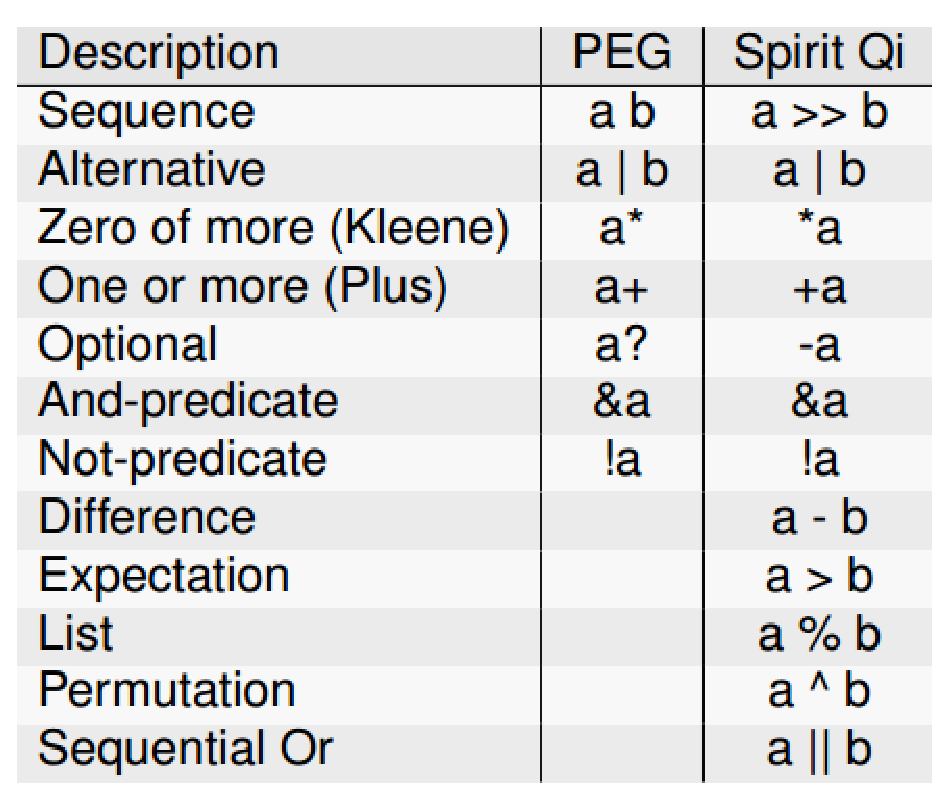
\includegraphics[height=6cm,
    angle=0]{./images/Boost_Spirit_operators.eps}}
  \caption{PEG (Parsing Expression Grammar) and its equivalent form in
  boost::spirit::qi}
  \label{fig:boost_spirit::qi_operators}
\end{figure}

Example: Write a parser that can detect a multi-line string, each line is the
form 'word : word'. Whenever we use \verb!phrase_parse()!, we need to provide a
$skip$ parsers as the last-argument, e.g \verb!space! is the skip parser here

\begin{verbatim}
#include <boost/spirit/include/qi_parse.hpp>

// the input string
std::string input( "foo : bar "
    "gorp : smart "
    "falcou : \"crazy frenchman\" "
    "arm8 : risc " );

// two iterators
std::string::iterator iter = input.begin();
std::string::iterator iter_end = input.end();

boost::spirit::qi::phrase_parse( iter, iter_end,
// ------ start parser -------
*( (alpha >> *alnum)
>> ':'
>> ('"' >> *( ~char_('"') ) >> '"')
|
(alpha >> *alnum)
)
// ------- end parser --------
, space );
\end{verbatim}

However, so far we haven't discussed how to retrived the information from the
input string, when the parsing is successful.


Example: We can define rules to simplify the parser passed to the
\verb!phrase_parse()! command. Consider the example above:
multiple lines, each with \verb!keyword: value! form. We use \verb!qi::rule! to
define the grammar, and parse the input string using \verb!parse_phrase()!.
Here, \verb!space_type! is the $skip$-parser.

\begin{verbatim}
qi::rule<iter_t, space_type> name;
name = alpha >> *alnum;

qi::rule<iter_t, space_type> quote;
quote = '"' >> *( ~char_('"') ) >> '"';
\end{verbatim}
Here, the rule needs an iterator \verb!iter_t!, and a skipper type to be used by
the rule \verb!space_type!.
\begin{verbatim}
std::string input( "foo : bar "
				"gorp : smart "
				"falcou : \"crazy frenchman\" "
				"arm8 : risc " );

typedef std::string::iterator iter_t;
iter_t iter = input.begin();
iter_t iter_end = input.end();

rule<iter_t, space_type> name = alpha >> *alnum;
rule<iter_t, space_type> quote = '"'
			>> *(~char_('"'))
			>> '"';

phrase_parse( iter, iter_end,
		// ------ start parser -------
	*( name >> ':' >> ( quote | name ) )
		// ------- end parser --------
		, space );
\end{verbatim}


%\cprotect\subsection[Using grammar class]{Using \verb!grammar! class} 
\subsection{Using 'grammar' class}

In the case the grammar is quite complicated, you can create your own parser as
a child of the \verb!boost::spirit::qi::grammar! class and using \verb!rule!
inside the grammar.

You should write your grammar first in PEG (Parsing Expression Grammar) which is
easy to understand. PEG is well-suited for parsing computer language, but not
for natural languages
\footnote{\url{http://en.wikipedia.org/wiki/Parsing_expression_grammar}}.

\begin{verbatim}
#include <boost/spirit/include/support_utree.hpp>
#include <boost/spirit/include/qi.hpp>
#include <boost/spirit/include/phoenix_core.hpp>
#include <boost/spirit/include/phoenix_operator.hpp>
#include <boost/fusion/include/adapt_struct.hpp>
#include <boost/assert.hpp>
#include <iostream>
#include <string>
#include <cstdlib>

using boost::spirit::qi;

template <typename Iter>
struct MyGrammar : grammar<Iter, space_type>
{
 //start = name of the starting rule
  MyGrammar() : MyGrammar::base_type(start)
  {
    start = *item;
    item = key >> ':' >> value;
    key = alpha >> *alnum;
    value = ('"' >> *(~char_('"')) >> '"')
            |
            *alnum;
  };

  rule<Iter, space_type> start;
  rule<Iter, space_type> item;
  rule<Iter, space_type> key;
  rule<Iter, space_type> value;
  
};   // IMPORTANT: Don't forget the semicolon here
\end{verbatim}

Now, we  can parse the input string, using \verb!space! as the $skip$ parser.
\begin{verbatim}
int main() {
  std::string input( "foo : bar "
		"gorp : smart "
		"falcou : \"crazy frenchman\" "
		"arm8 : risc " );

  typedef std::string::iterator iter_t;
  iter_t iter = input.begin();
  iter_t iter_end = input.end();

  MyGrammar<iter_t> list_grammar;

  boost::spirit::qi::phrase_parse( iter, iter_end,
        list_grammar,
        space );
		
}
\end{verbatim}



\subsection{Action: Get parsed results}

What if we want to get the parsed results, i.e. we want to keep a list of
'key' and its associated 'value'. That is we need to use the attribute type
associated with each parsers, Fig.\ref{fig:boost_spirit_qi_attribute-type}. The
argument(s) to \verb!parse()! or \verb!parse_phrase()! counting from the
fourth-argument to the one before the last argument, returns the value(s) of the
attribute type associated with the parser.  

Example: here, we use two variables to save the attribute values for two
parsers.

\begin{verbatim}
std::string input( "cosmic pizza" );
std::string::iterator iter = input.begin();
std::string::iterator end_iter = input.end();
std::string result1;
std::string result2;

boost::spirit::qi::parse( iter, end_iter,
		*(~char_(' ')) >> ' ' >> *char_,
		result1,
		result2 );

\end{verbatim}



If you look at the way a parser is defined, the second template type, i.e. T, is
the type of the attribute.
\begin{verbatim}
template <typename P, typename T>
MyGrammar : qi::grammar<P, T> 
{
  ...
}
\end{verbatim}

\begin{figure}[hbt]
  \centerline{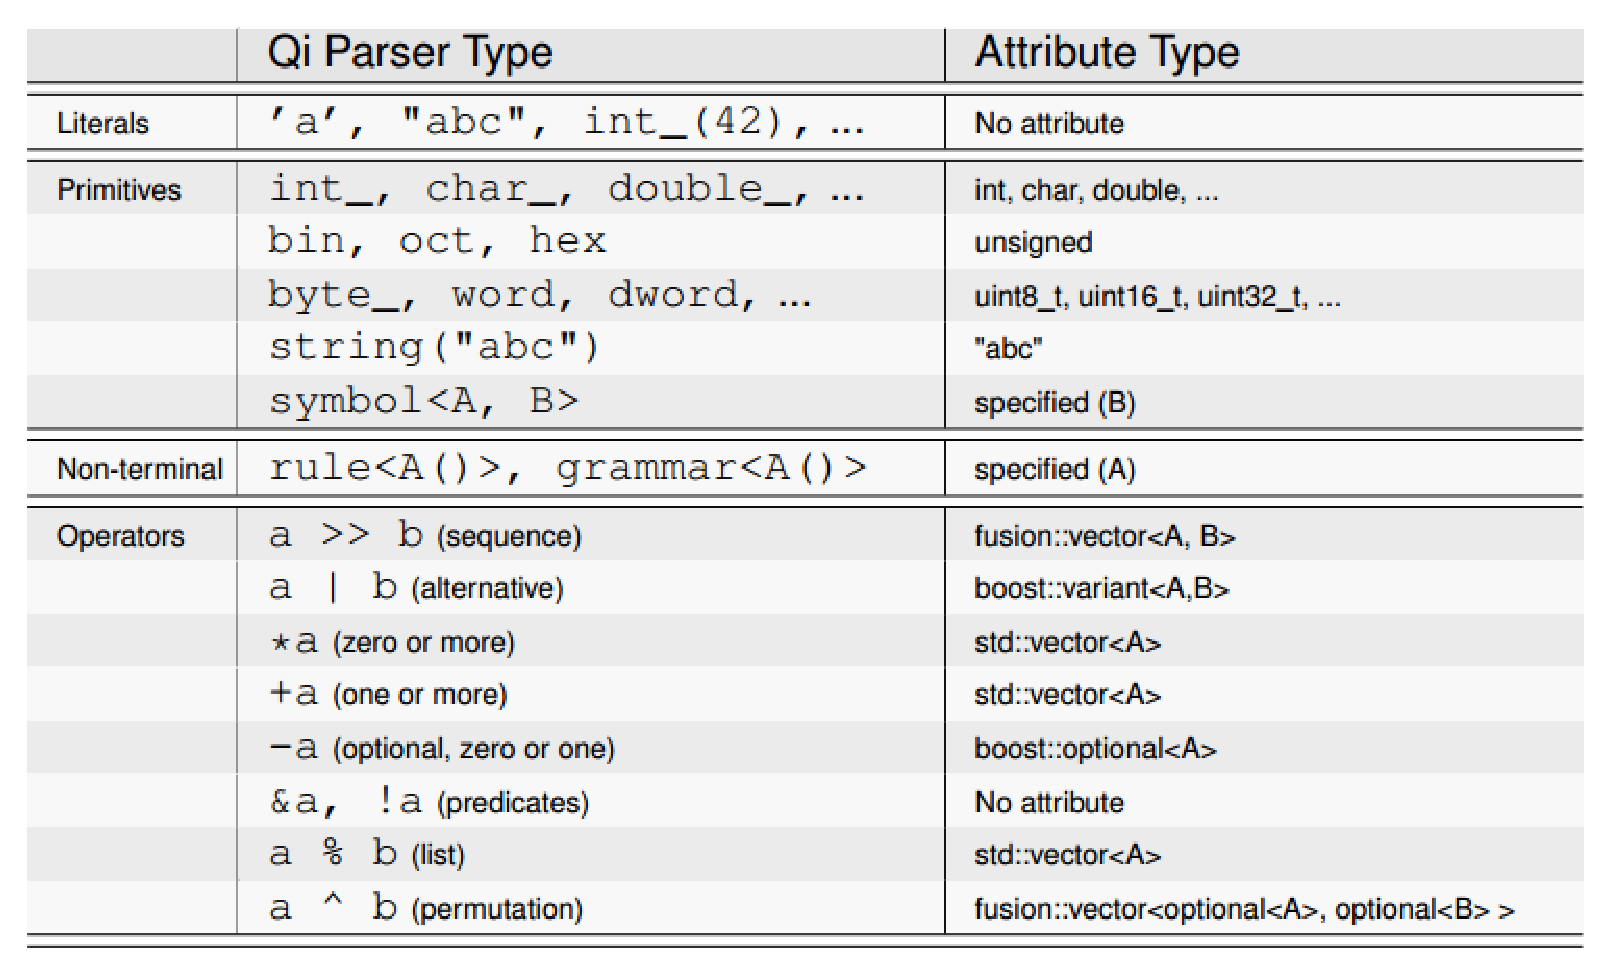
\includegraphics[height=7cm,
    angle=0]{./images/Boost_Spirit_attribute-type.eps}}
\caption{Attribute type associated with primitives parsers}
\label{fig:boost_spirit_qi_attribute-type}
\end{figure}

\subsubsection{Return integer}
 
A simple example below return the integer value of the string, if parsing is
successful.
\begin{verbatim}
std::string input( "1234" );
std::string::iterator iter = input.begin();
std::string::iterator end_iter = input.end();
int result;
parse( iter, end_iter,
        int_,
        result );
\end{verbatim}

NOTE: Compatible attribute type can also be used to get the result, e.g
std::string is compatible with std::vector<char>
attribute of the \verb!*char_! parser.
\begin{verbatim}
std::string input( "pizza" );
std::string::iterator iter = input.begin();
std::string::iterator end_iter = input.end();
std::string result;
parse( iter, end_iter,
		*char_,
		result );
\end{verbatim}

\subsubsection{Return a pair of strings}

If the grammar contains of 2 types of token, we can use more than one parsers
(separated by \verb!>>!, and extract the string value from each parser by using
more than one variable , to get the corresponding associated attrubute
\begin{verbatim}
std::string input( "cosmic pizza" );
std::string::iterator iter = input.begin();
std::string::iterator end_iter = input.end();
std::string result1;
std::string result2;

boost::spirit::qi::parse( iter, end_iter,
		*(~char_(' ')) >> ' ' >> *char_,
		result1,
		result2 );
\end{verbatim}
Here \verb!result1! keep the value for \verb!*(~char_(' '))!, the attribute for
' ' is \verb!unused! or it has no attribute, and \verb!result2! keeps the value
for \verb!*char_!. 

If we want to use $skip$ parser, we need to make sure the white space is not
removed before exttracting the tokens.
\begin{verbatim}
// with skip parser, we don't need to use ' ' token.
// However, you will get unexpected result here
// as result1 keep the 2 words without spaces between 
// and result2 is empty
boost::spirit::qi::phrase_parse( iter, end_iter,
		*(~char_(' ')) >> ' ' >> *char_, ascii:space_type
		result1,
		result2 );

// to resolve the issue
// the solution is lexeme[ ... ]
// any space between will not be removed before applying the sub-parser
boost::spirit::qi::phrase_parse( iter, end_iter,
		lexeme[*(~char_(' '))] >>  *char_, ascii:space_type
		result1,
		result2 );
\end{verbatim}

\subsubsection{Return a vector of strings}

\subsubsection{Return a map of <string, string>}

Again, the two string can be compatible to a map of two string. 
\begin{verbatim}
std::pair<std::string, std::string> result;
parse( iter, end_iter,
		*(~char_(' ')) >> ' ' >> *char_,
		result );
\end{verbatim}

Example: put into the vector
\begin{verbatim}
std::list<int> list;

void got_it (int n) { list.push_back (n); }

*('{' >> lit("0x") >> hex[&got_it] >> '}'))
\end{verbatim}
The idea is simple: when a hexadecimal number is recognized, call a function
which pushes the number onto a list"
\footnote{\url{http://climbing-the-hill.blogspot.com/2010/05/boost-your-spirits.html}}.

Example: Here, we use <map>
\begin{verbatim}
std::map< std::string, std::string > key_value_map;

std::string input( "foo : bar ,"
				"gorp : smart ,"
				"falcou : \"crazy frenchman\" " );

typedef std::string::iterator iter_t;
iter_t iter = input.begin();
iter_t iter_end = input.end();

rule<iter_t, std::string(), space_type> name = alpha >> *alnum;
rule<iter_t, std::string(), space_type> quote = '"'
				>> lexeme[ *(~char_('"')) ]
				>> '"';
rule<iter_t, std::pair<std::string, std::string>(), space_type>
			item = name >> ':' >> ( quote | name );

std::map< std::string, std::string > key_value_map;

phrase_parse( iter, iter_end,
			item % ',',
			space,
			key_value_map );
\end{verbatim}
NOTE: How the starting rule \verb!item! has the associated attribute type of
\verb!std::pair<std::string, std::string>()!, and its two sub-rules \verb!name!
and \verb!quote! has the associated attribute types as \verb!std::string()!.

Example: Fig.\ref{fig:Boost_Spirit_example_1} also include the printint out
parsed result using \verb!std::for_each! loop. \textcolor{red}{QUESTIONS: What
is }\verb!phx::at_c<0>(arg1)!
\footnote{\url{http://www.boost.org/doc/libs/1_46_1/libs/fusion/doc/html/fusion/adapted/std__pair.html}}.
\verb!at_c<N>(seq)! returns the $N$-th element from the beginning of the
sequence.

\begin{verbatim}
std::pair<int, std::string> p(123, "Hola!!!");
std::cout << at_c<0>(p) << std::endl;
std::cout << at_c<1>(p) << std::endl;
std::cout << p << std::endl;

vector<int, int, int> v(1, 2, 3);
assert(at_c<1>(v) == 2);
\end{verbatim}


\begin{figure}[hbt]
  \centerline{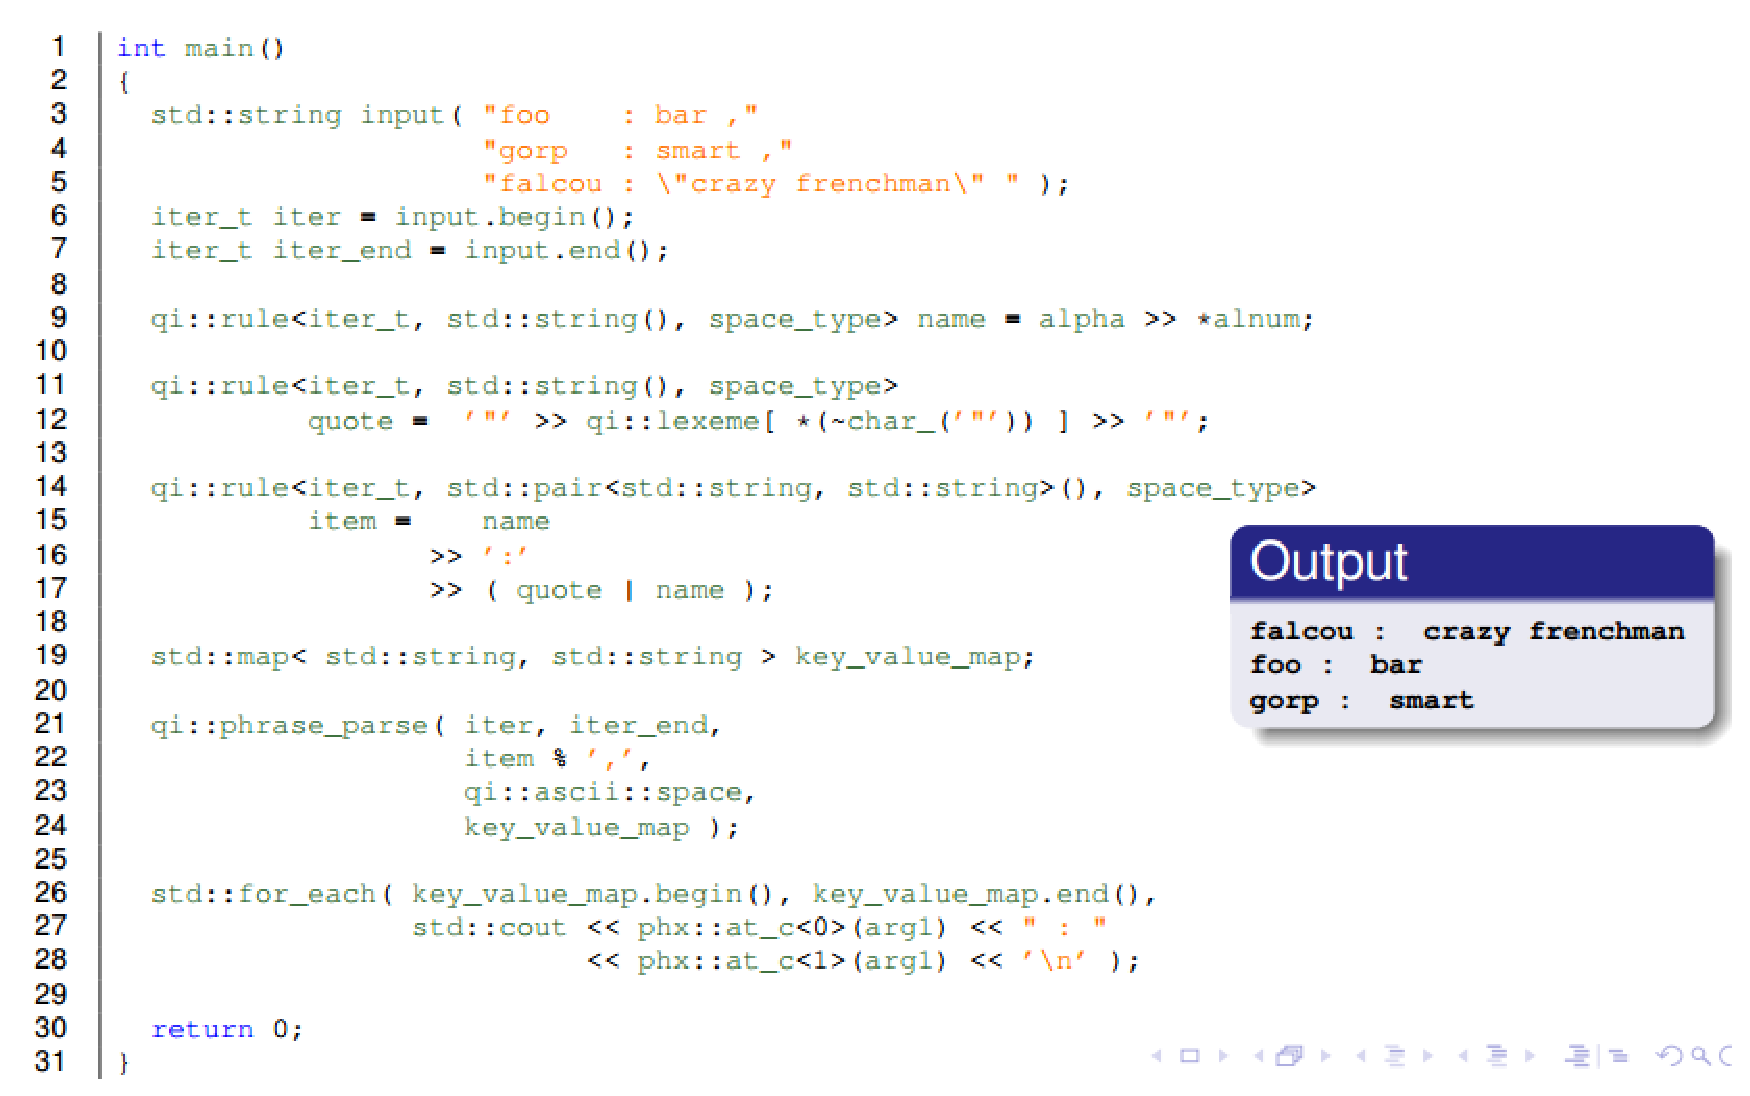
\includegraphics[height=8cm,
    angle=0]{./images/Boost_Spirit_example_1.eps}}
\caption{A complete example of using Boost::spirit::qi}
\label{fig:Boost_Spirit_example_1}
\end{figure}

\subsubsection{Return a struct}

There are two ways: the not-a-smart-way is to create a struct with a
proper construction. The second way is discussed in the next section, using
Boost.Fusion.

\subsubsection{Return a struct (using Boost.Fusion)}


First we create a struct that we want to store the parsed data
\begin{verbatim}
namespace myclient {
  struct employee
  {
  int age;
  std::string firstname;
  std::string lastname;
  double salary;
//  std::map<std::string, std::string> some_record;
  }
}
\end{verbatim}
NOTE: The problem of using a comma (,) in the type, which when pass to macro
expansion it can give you errors like
\begin{verbatim}
macro "BOOST_FUSION_ADAPT_STRUCT_FILLER_0" passed 3 arguments, but takes just 2
\end{verbatim}
when you do something
\begin{verbatim}
BOOST_FUSION_ADAPT_STRUCT(TestStruct, (int, myint)(double, mydouble)
       (std::pair<std::string, std::string>, some_record));
\end{verbatim}
To resolve this problem, just use \verb!typedef! to define a new name, and then
use the alias name for the data type.
\begin{verbatim}
typedef std::pair<std::string, std::string> my_type_t;

BOOST_FUSION_ADAPT_STRUCT(TestStruct, (int, myint)(double, mydouble)
       (my_type_t, some_record));
\end{verbatim}


Then, at the global namespace, use Boost.Fusion
\begin{verbatim}
BOOST_FUSION_ADAPT_STRUCT(TestStruct, (int, myint)(double, mydouble));
\end{verbatim}

Then, next in the \verb!myclient! namespace, we define
\begin{verbatim}
template <typename Iterator, typename Skipper>
struct MyGrammar : qi::grammar<Iterator, TestStruct(), Skipper> {
    MyGrammar() : MyGrammar::base_type(mystruct) {
        mystruct = qi::int_ >> ":" >> qi::double_;
    }
    qi::rule<Iterator, TestStruct(), Skipper> mystruct;
};
\end{verbatim}

Finally, you can use it
\begin{verbatim}
int main() {
    typedef std::string::const_iterator It;
    const std::string input("2: 3.4");
    It it(input.begin()), end(input.end());

    MyGrammar<It, qi::space_type> gr;
    TestStruct ts;

    if (qi::phrase_parse(it, end, gr, qi::space, ts) && it == end)
        std::cout << ts.myint << ", " << ts.mydouble << std::endl;

    return 0;
}
\end{verbatim}

\subsection{Attribute parsing - compatibility}
\label{sec:associate_attribute_compatible-type}

\begin{verbatim}
a: char, b: std::vector<char> 
  -->  ( a >> b ): std::vector<char>

a: unused, b: vector<char>, c: unused 
  --> ( a >> b >> c): std::vector<char>

a: string, b: string 
  --> ( a | b): variant<string, string> ! string

a: string, b: unused, c: string 
  --> ( a >> b >> c): tuple<string, string>

a: std::pair<string, string> 
  --> ( a % b ): vector< std::pair<string, string> >
    
\end{verbatim}


\subsection{Minimum headers to use}

When we implement the parser
\begin{verbatim}
#include <boost/spirit/include/qi.hpp>
#include <boost/spirit/include/phoenix.hpp>
#include <boost/fusion/include/adapt_struct.hpp>
\end{verbatim}

When we use the parser, we need
\begin{verbatim}
#include <boost/fusion/include/std_pair.hpp>
\end{verbatim}
This is important if your parser using \verb!std::pair< , >!.

\subsection{Detecting error when parsing}

\url{http://boost-spirit.com/home/articles/qi-example/tracking-the-input-position-while-parsing/}



\subsection{C++ preprocessor using Qi::Classic}

\url{http://www.codeproject.com/Articles/3853/Wave-a-Standard-conformant-C-preprocessor-library}

\section{High-order function objects}

To write code more concise, expressive and readable. 

\section{Smart pointers}

Smart pointers provide automatic lifetime management of objects and simplify
resource sharing. This is now part of C++11 

\section{Conversion to containers and data structures}


\section{Regular expression: Boost.Regex, Boost.Tokenizer}

If we have sophisticated text processing, we can use Boost.Regex, 
Boost.Tokenizer, or Boost.Spirit. 

\section{Function objects defined at the call site: Boost.Bind and
Boost.Lambda}

For functional programming, we can use \verb!Boost.Lambda!.

\section{Flexible callbacks: Boost.Function}

\section{Manage signals + slots: Boost.Signals}

\section{Convert text and numbers: Boost.lexical\_cast}

To convert between text and numbers, or between any streamable types, we use
\verb!Boost.lexical_cast!


\section{Math: Boost.Math}
\label{sec:boost_math}


\url{http://www.boost.org/doc/libs/1_53_0/libs/math/doc/html/index.html}

\section{Random: Boost.Random}


\section{Rational number: Boost.Rational}

\section{Complex number: Boost.Quaternion}

Quaternion provides an efficient way to parameterize rotation in 3D and 4D.

\url{http://www.boost.org/doc/libs/1_41_0/libs/math/doc/quaternion/html/}

\section{Multi-dimensional array: Boost.MultiArray}



\section{Graph: Boost.Graph}

\section{Timer/IO utilities: Boost.Chrono}
\label{sec:Boost-Chrono}
\label{sec:Chrono-library}
\label{sec:Boost.Chrono}

\url{http://www.boost.org/doc/libs/1_58_0/doc/html/chrono.html}
\begin{lstlisting}
// Include all of Chrono files
#include <boost/chrono.hpp>

\end{lstlisting}


Some features is now part of C++11 \verb!#include! \verb!<chrono>! - Sect.\ref{sec:chrono-header-file}
   
NOTE: Boost Chrono has I/O, rounding and many other clock utilities that C++11
doesn't have. So, we may still want to use Boost Chrono in these situations.

\section{Utilities}


\begin{verbatim}
#include <boost/utility.hpp>
\end{verbatim}



\subsection{result\_of}
\label{sec:result_of-BOOST}

\verb!boost::result_of<>! =  \verb!std::result_of!

It was introduced in Boost, and then included into C++ TR1, then C++0x, and now
is part of C++11 standard.
In C++11, we can use a similar language feature called \verb!decltype! which is
an entirely new thing in C++0x, does not restrict only to return type of a
function, and is a language feature.

In C++0x, \verb!result_of! is implemented based on \verb!decltype!
\begin{verbatim}
 template<typename _Signature>
    class result_of;

  template<typename _Functor, typename... _ArgTypes>
    struct result_of<_Functor(_ArgTypes...)>
    {
      typedef
        decltype( std::declval<_Functor>()(std::declval<_ArgTypes>()...) )
        type;
    };
\end{verbatim}

\url{https://www.boost.org/doc/libs/1_42_0/boost/utility/result_of.hpp}

The class template \verb!result_of! helps determine the type of a call
expression.
For example, given an lvalue (Sect.\ref{sec:lvalue}) f of type F and lvalues
t1, t2, ..., tN of types T1, T2, ..., TN, respectively, the type
\verb!result_of<F(T1, T2, ..., TN)>::type! defines the result type of the
expression f(t1, t2, ...,tN).

\begin{verbatim}

\end{verbatim}

This implementation permits the type F to be a function pointer, function
reference, member function pointer, or class type.

Boost::\verb!result_of! has, by default, N may be any value between 0 and 16.
To change the upper limit, define the macro \verb!BOOST_RESULT_OF_NUM_ARGS! to the maximum value for N, as defined in 
\verb!boost/utility/result_of.hpp! file.



\begin{verbatim}
//namespace boost

template<typename F> struct result_of;
\end{verbatim}

\section{C++ and other language}

\subsection{Python: Boost.Python}

